\documentclass[12pt,a4paper]{article}

\usepackage[utf8]{inputenc}
\usepackage[T2A]{fontenc}
\usepackage[ukrainian]{babel}
\usepackage{geometry}
\geometry{
    left=2cm,
    right=2cm,
    top=2cm,
    bottom=2cm
}

\usepackage[table]{xcolor}
\usepackage{amsmath}
\usepackage{graphicx}
\usepackage{subcaption}
\usepackage{multirow}
\usepackage{makecell}
\usepackage{pdflscape}
\usepackage{array}
\newcolumntype{C}[1]{>{\centering\arraybackslash}m{#1}}

\usepackage{minted}

\usemintedstyle{vs}
\setminted{linenos, breaklines, frame=single, fontsize=\small}

\RecustomVerbatimCommand{\VerbatimInput}{VerbatimInput}{
    breaklines=true,
    breaksymbolleft={}
}

\usepackage[
  unicode,
  pdftitle={ІО-41, Давидчук А.М., АК. Частина 1, Лабораторна робота №3},
  pdfauthor={Давидчук Артем},
  pdfsubject={Архітектура Комп'ютерів. Частина 1}
]{hyperref}

\begin{document}

    \begin{titlepage}

        \begin{center}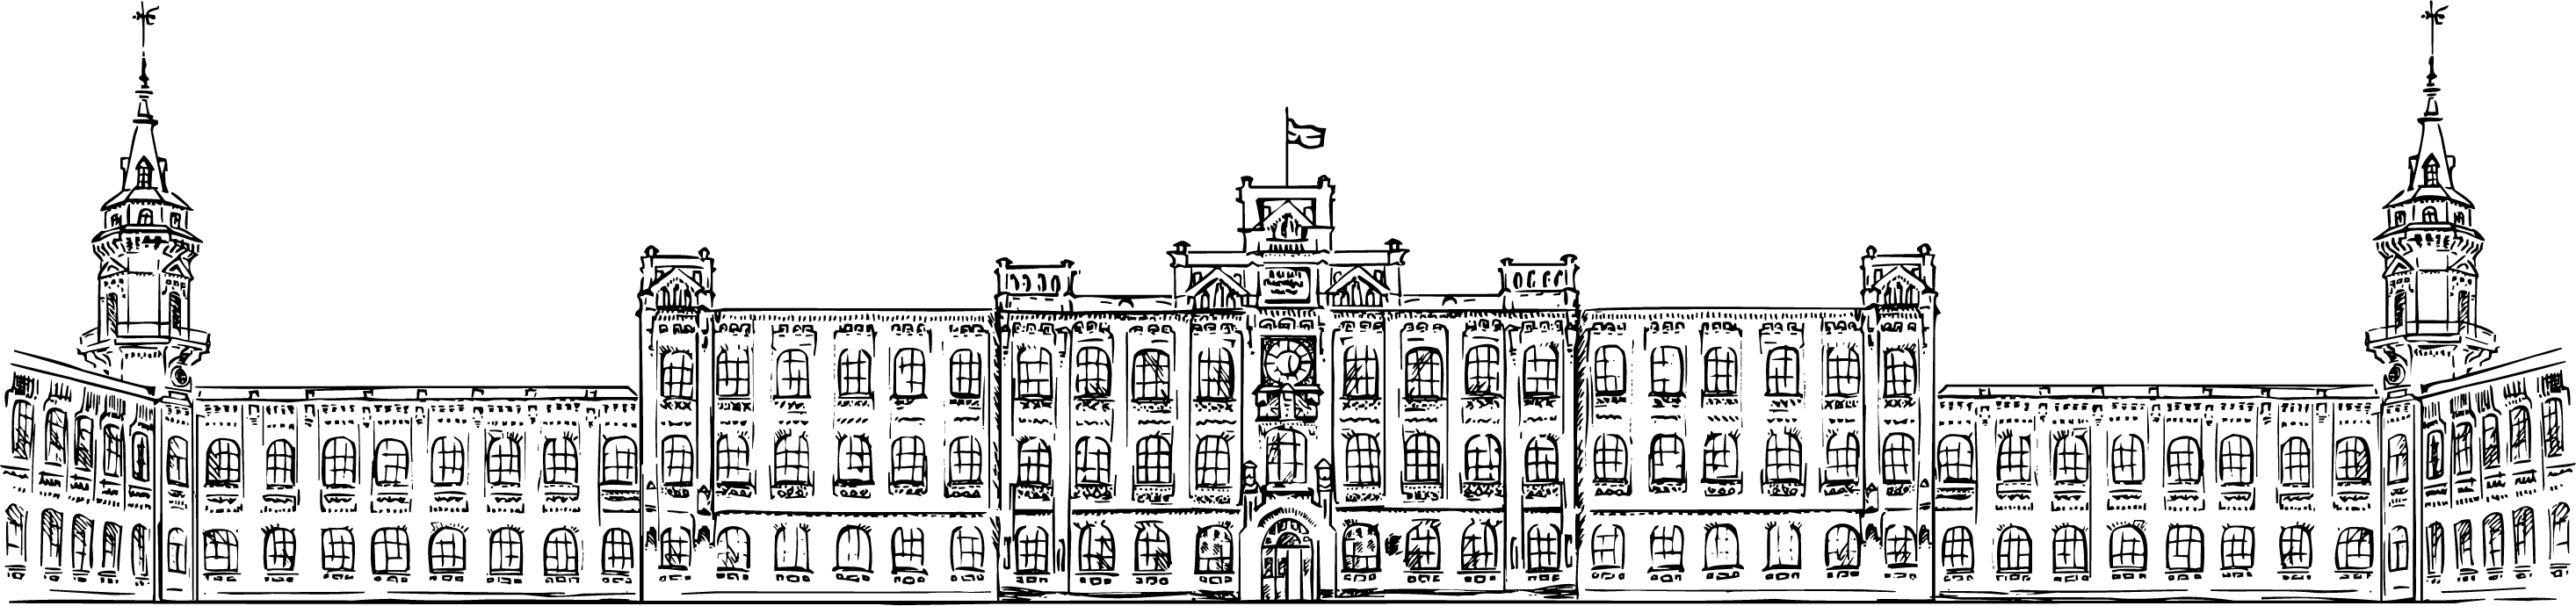
\includegraphics[width=0.7\textwidth]{../../../TITLES/letterhead.png}\end{center}

        \begin{center}
            \large Національний технічний університет України\\
            «Київський політехнічний інститут імені Ігоря Сікорського»\\[1em]
            Факультет інформатики та обчислювальної техніки\\
            Кафедра обчислювальної техніки
        \end{center}

        \vfill

        \begin{center}
            \textbf{\LARGE Архітектура Комп'ютерів. Частина 1}\\[2em]
            \textbf{\Large Лабораторна робота №3}\\[0.5em]
            «Перетворення даних в ЕОМ на мікропрограмному рівні» 
        \end{center}

        \vfill

        \begin{flushright}
            Виконав: студент 2 курсу ФІОТ, гр. ІО-41\\
            \textit{Давидчук А. М.}\\
            Залікова книжка № 4106\\[1em]
            Перевірив: \textit{Верба О.\,А.}
        \end{flushright}

        \vfill

        \begin{center}Київ --- 2026\end{center}

    \end{titlepage}

    \noindent
    \textbf{\underline{Тема:}} «Перетворення даних в ЕОМ на мікропрограмному рівні» .

    \vspace{1em}

    \noindent
    \textbf{\underline{Мета:}} вивчити архітектуру ЕОМ, що містить блок мікропрограмного керування
    і арифметико-логічний пристрій з зосередженою логікою та двухадресним надоперативним запам'ятовуючим пристроєм (НОЗП),
    одержати навики розробки мікропрограм.

    \begin{center} \textbf{\large Порядок виконання роботи} \end{center}

    \newpage

    \begin{center} \textbf{\large Хід роботи} \end{center}

    Мій номер залікової книжки: 4106, що у двіковому вигляді є 0001 0000 0000 1010.
    Звідси $a_7 = 0, a_6 = 0, a_5 = 0, a_4 = 1, a_3 = 0, a_2 = 1, a_1 = 0$. Тобто я маю такий варіант:

    \begin{table}[h!]
    \centering
    \begin{subtable}[t]{0.38\textwidth}
    \centering
    \begin{tabular}{|c|c|c|}
    \hline
    $a_5$ & $a_4$ &
    \begin{tabular}[c]{@{}c@{}}
    Спосіб\\
    множення\\
    (при $g=1$)
    \end{tabular} \\
    \hline
    0 & 0 & 4 \\
    \rowcolor{yellow!50}
    0 & 1 & 1 \\
    1 & 0 & 2 \\
    1 & 1 & 3 \\
    \hline
    \end{tabular}
    \caption{Спосіб множення}
    \end{subtable}
    \hfill
    \begin{subtable}[t]{0.42\textwidth}
    \centering
    \begin{tabular}{|c|c|c|}
    \hline
    $a_6$ & $a_1$ &
    \begin{tabular}[c]{@{}c@{}}
    Арифметична\\
    операція\\
    (при $g=0$)
    \end{tabular} \\
    \hline
    \rowcolor{yellow!50}
    0 & 0 & $2^2X - 2^{-1}Y$ \\
    0 & 1 & $2^{-1}X + 2^2Y$ \\
    1 & 0 & $2^3X - 2Y$ \\
    1 & 1 & $2^2X + 2^{-1}Y$ \\
    \hline
    \end{tabular}
    \caption{Арифметична операція}
    \end{subtable}

    \vspace{2em}

    \begin{subtable}[t]{0.42\textwidth}
    \centering
    \begin{tabular}{|c|c|c|c|c|}
    \hline
    $a_3$ & $a_2$ & $X$ & $Y$ & $Z$ \\
    \hline
    0 & 0 & ДК & ДК & ПК \\
    \rowcolor{yellow!50}
    0 & 1 & ПК & ПК & ДК \\
    1 & 0 & ПК & ДК & ПК \\
    1 & 1 & ДК & ПК & ДК \\
    \hline
    \end{tabular}
    \caption{Форма подання чисел}
    \end{subtable}
    \hfill
    \begin{subtable}[t]{0.38\textwidth}
    \centering
    \begin{tabular}{|c|c|c|c|}
    \hline
    $a_7$ & $a_1$ & $X$ & $Y$ \\
    \hline
    \rowcolor{yellow!50}
    0 & 0 & 7  & -5 \\
    0 & 1 & -7 & 9 \\
    1 & 0 & -9 & -5 \\
    1 & 1 & 7  & -6 \\
    \hline
    \end{tabular}
    \caption{Значення операндів}
    \end{subtable}

    \caption{Таблиці вибору функцій і тестових даних}
    \end{table}

    А ознака $g$ визначається у вихідному стані значенням розряду з двійковим номером $a_3 a_2 a_1 = 010 = 2$ регістра <RN стану процесора.

    \vspace{1em}

    Загальна структура ЕОМ:

    \begin{figure}[h!]
        \centering
        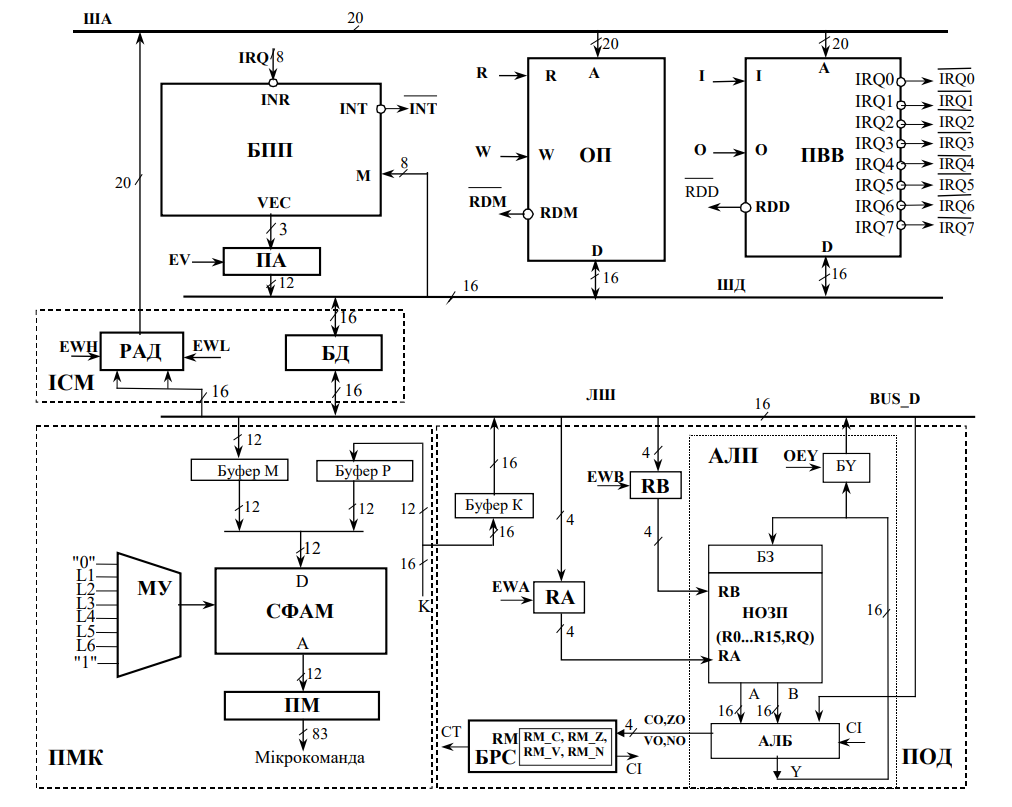
\includegraphics[width=0.7\linewidth]{media/eom.png}
    \end{figure}

    \newpage

    Надам операційні схеми для функції

    \[
    Z =
    \begin{cases}
    X \cdot Y, & \text{якщо } g = 1,\\
    2^{2}X - 2^{-1}Y, & \text{якщо } g = 0.
    \end{cases}
    \]

    \begin{figure}[h!]
        \centering
        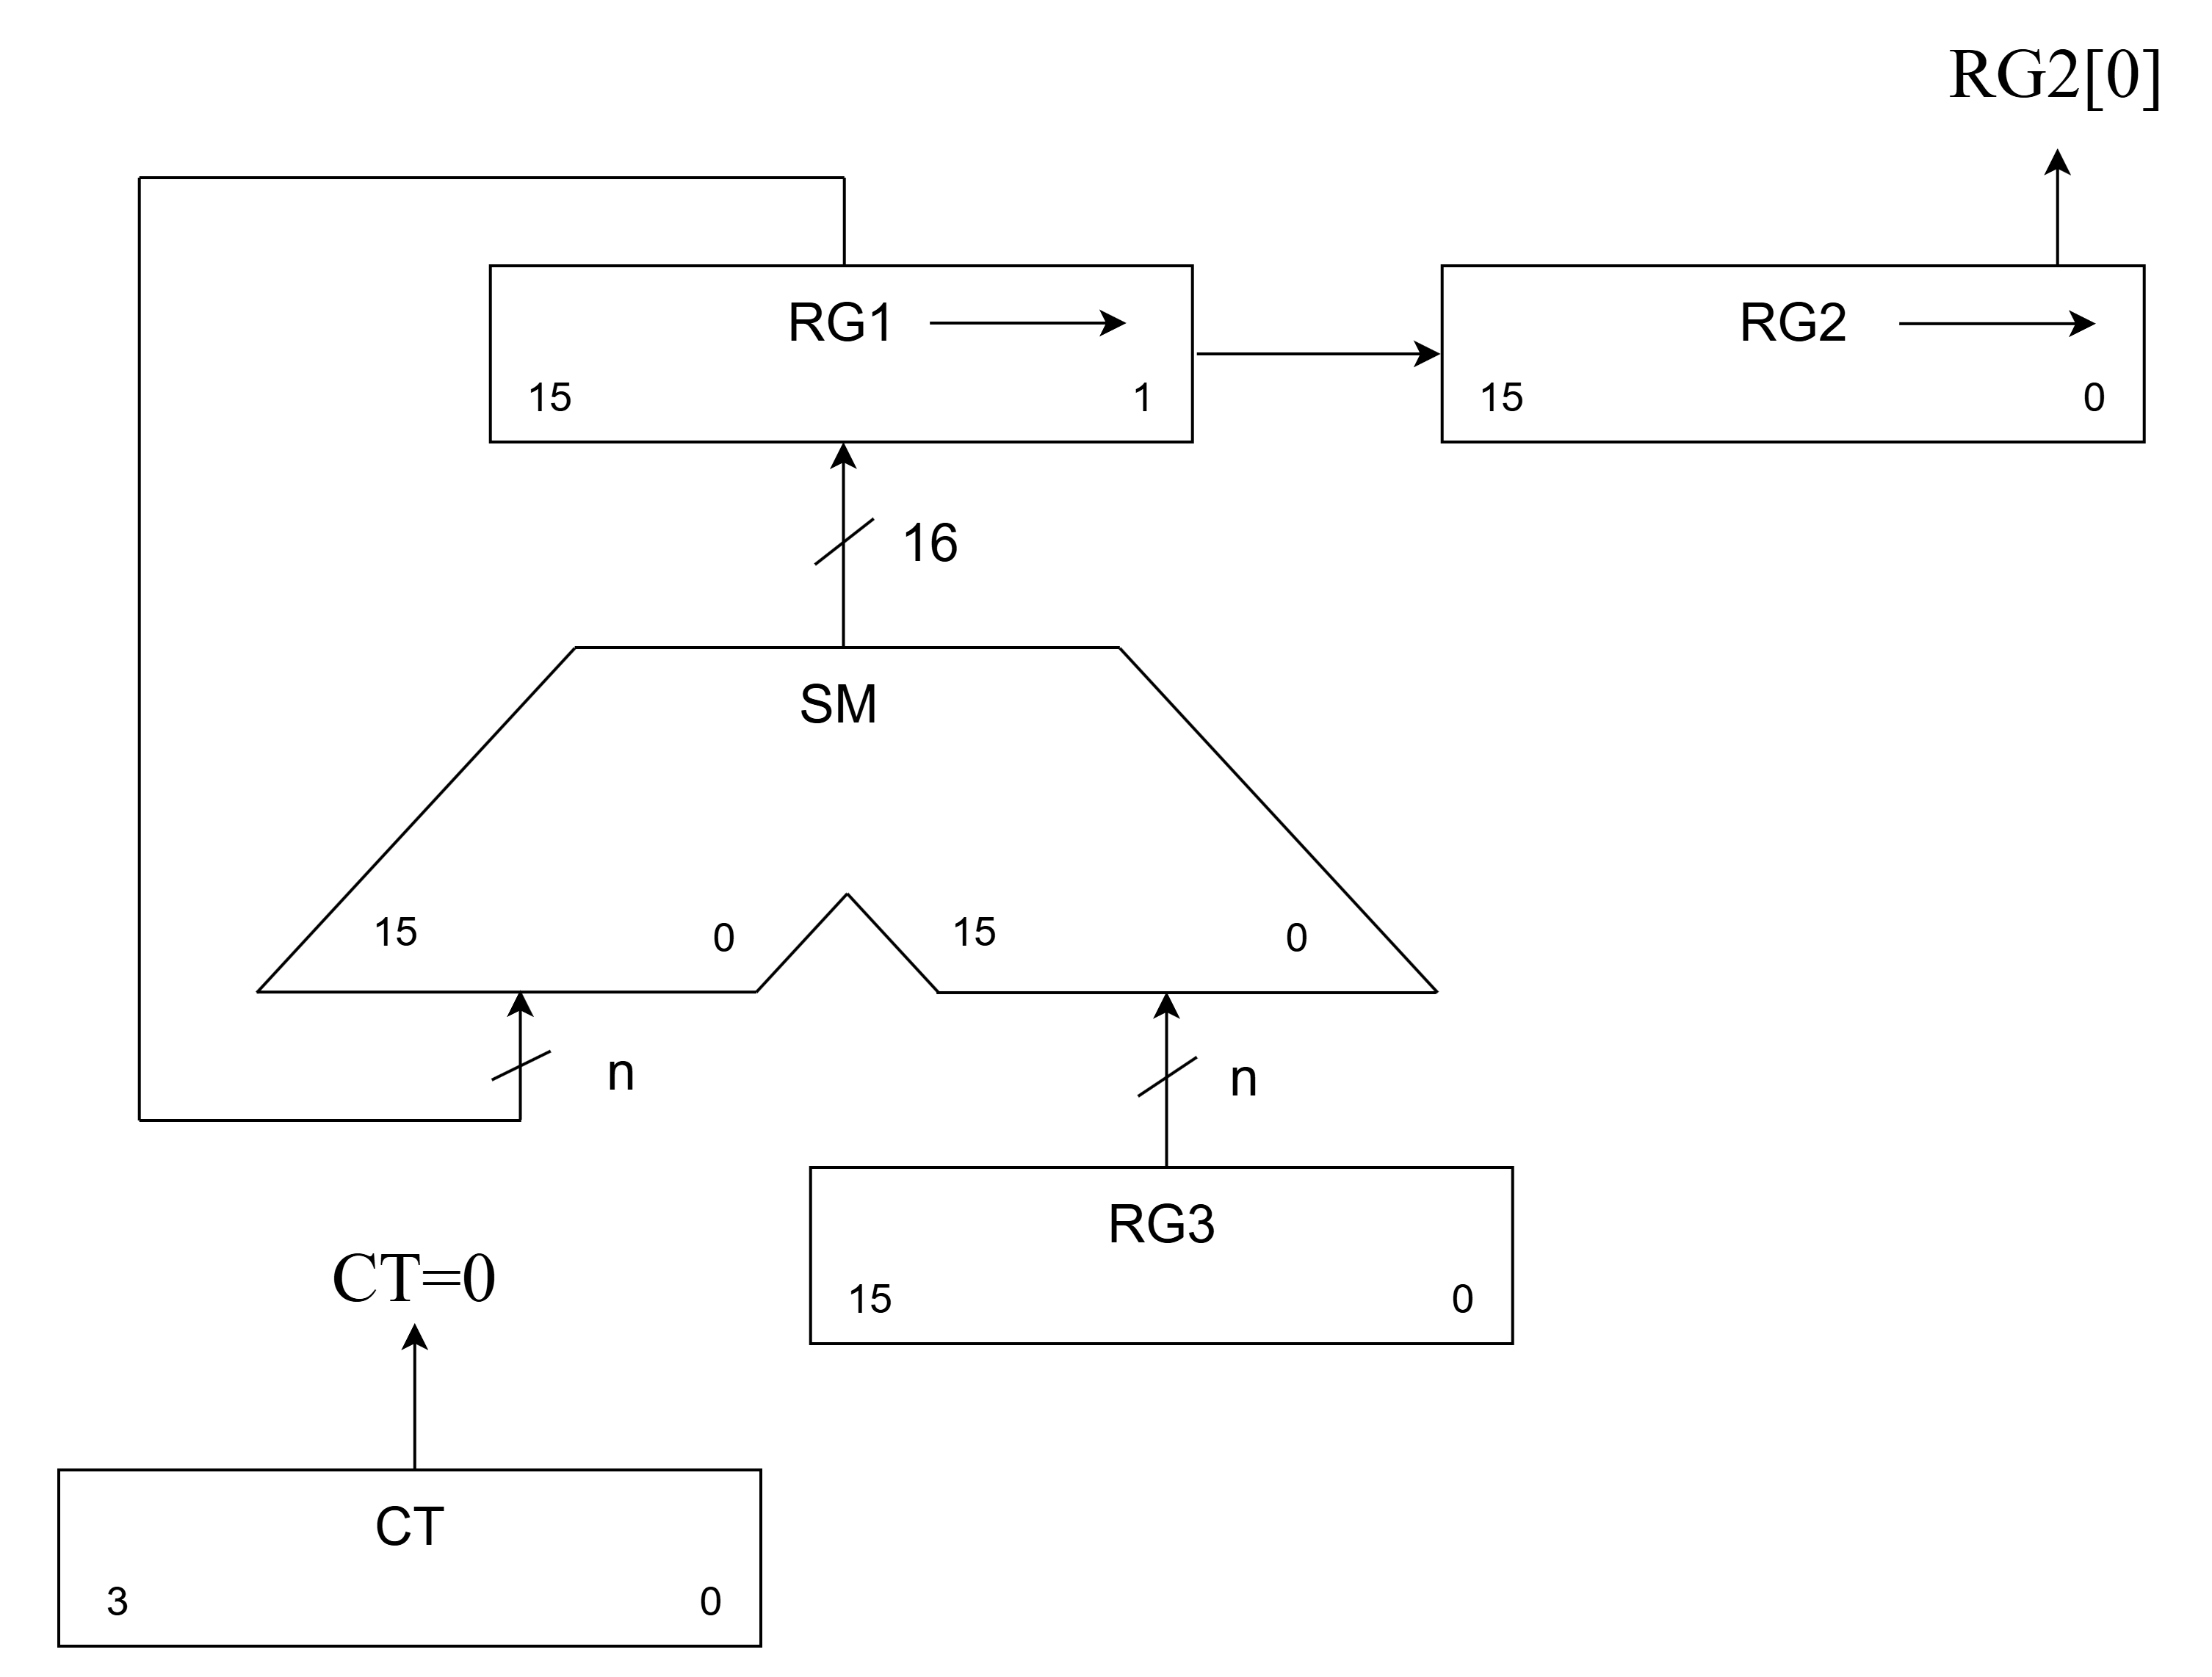
\includegraphics[width=0.6\linewidth]{media/multi.png}
        \caption{Операційна схема множення 1 способом}
    \end{figure}

    \begin{figure}[h!]
        \centering
        
\includegraphics[width=0.5\linewidth]{media/func.png}
        \caption{Операційна схема функції $2^{2}X - 2^{-1}Y$}
    \end{figure}

    \newpage

    \noindent
    Наведемо функціональні мікроалгоритми для обчислення функцій:

    \begin{figure}[h!]
        \centering
        
\includegraphics[width=0.8\linewidth]{media/alg1.png}
    \end{figure}

    \newpage

    \noindent
    Таблиця станів регістрів при $g = 1$ (множення 1 способом):

    \newpage

    \noindent
    Таблиця станів регістрів при $g = 0$ (обчислення функції $2^{2}X - 2^{-1}Y$):

    \vspace{1em}

    \noindent
    Число $X = 7$ в ДК: 00.00000000000111, число $Y = -5$ в ДК: 11.11111111111011

    \vspace{1em}

    \begin{table}[h!]
        \centering
        \renewcommand{\arraystretch}{1.3}
        \begin{tabular}{|c|c|c|c|p{4.5cm}|}
            \hline
            \textbf{№} &
            \makecell{\textbf{RG8} \\[0.3em] 15 - 0} &
            \makecell{\textbf{RG9} \\[0.3em] 15 - 0} &
            \makecell{\textbf{RG13} \\[0.3em] 15 - 0} &
            \textbf{Мікрооперації} \\
            \hline
            \textbf{0} &
            \makecell[l]{0000000000000111} &
            \makecell[l]{1111111111111011} &
            \makecell[l]{0000000000000000} &
            \makecell[l]{
                \texttt{RG13 := 0..00;} \\
                \texttt{RG8 := X;} \\
                \texttt{RG9 := Y;}
            } \\
            \hline

            \textbf{1} &
            \makecell{0000000000000111\\[1em] \textit{Після зсуву:}\\ 0000000000001110} &
            \makecell{1111111111111011\\[1em] \textit{Після зсуву:}\\ 1111111111111101} &
            \empty &
            \makecell[l]{
                \texttt{RG8 := L(RG8).0} \\
                \texttt{RG9 := 1.R(RG9)}
            } \\
            \hline

            \textbf{2} &
            \makecell{0000000000001110\\[1em] \textit{Після зсуву:}\\ 0000000000011100} &
            \empty &
            \empty &
            \makecell[l]{
                \texttt{RG8 := L(RG8).0}
            } \\
            \hline

            \textbf{3} &
            \empty &
            \empty &
            \makecell[l]{
            \(
            \begin{array}{r} % r - вирівнюємо вправо для акуратності
            +0000000000011100 \\
            \ \ 0000000000000010 \\
            \ \ 0000000000000001 \\
            \hline
            0000000000011111
            \end{array}
            \)
            } &
            \makecell[l]{
                \texttt{RG13 := RG8 + !RG9 +} \\
                \texttt{\quad + D;}
            } \\
            \hline
        \end{tabular}
    \end{table}

    Отримали число $Z = 00.00000000011111$ в ДК, що дорівнює 31 в десятковій, та 1F в шістнадцятковій системі числення.

    \vspace{1em}

    \noindent
    Запишемо код мікроассемблера:

    \inputminted{text}{src/work.asm}

    \noindent
    Та продемонструємо вивід програми (при різних режимах $g$):

    \begin{figure}[h!]
        \centering
        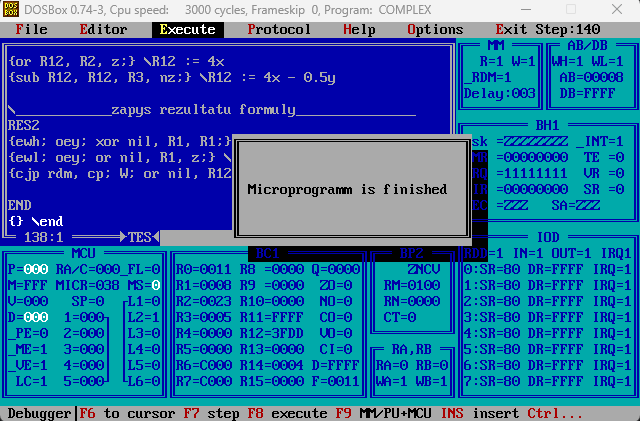
\includegraphics[width=0.8\linewidth]{media/multi_res.png}
        \caption{Результат множення}
    \end{figure}

    \begin{figure}[h!]
        \centering
        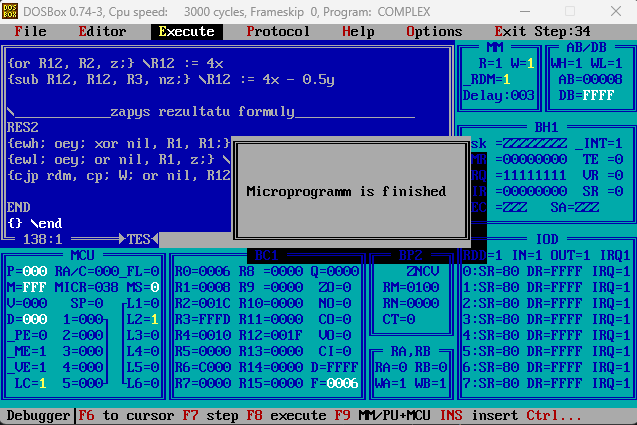
\includegraphics[width=0.8\linewidth]{media/func_res.png}
        \caption{Результат обчислення функції}
    \end{figure}

    Для множення, відповідь вийшла FFFF 3FDD, що дорівнює значенню FFFF FFDD, раніше обчисленим (тут просто особливість маски на другому регістрі), а під час обчислення функції відповідь дорівнюж 001F, що також співпадає із раніше обчисленим. Всі ці числа вже подані в ДК. Як бачимо, результати співпадають.

    \begin{center} \textbf{\large Висновок}\end{center}

    У ході виконання лабораторної роботи було досліджено перетворення даних в ЕОМ на мікропрограмному рівні та закріплено принципи роботи архітектури, що містить блок мікропрограмного керування, арифметико-логічний пристрій із зосередженою логікою та двоадресний НОЗП. Для заданого варіанта було визначено функцію обчислення, форму подання операндів і результату, а також спосіб множення: при $g = 1$ реалізується множення $X \cdot Y$ першим способом, а при $g = 0$ обчислюється вираз $2^{2}X - 2^{-1}Y$.

    У процесі роботи було побудовано операційні схеми та функціональний мікроалгоритм для обох режимів роботи, складено таблиці станів регістрів і розроблено мікропрограму для виконання заданих перетворень. Окрему увагу було приділено аналізу знаків операндів, переходу між прямим і додатковим кодами, виконанню зсувів, додавання, віднімання та запису результату до оперативної пам'яті у додатковому коді.

    Результати моделювання підтвердили правильність розробленої мікропрограми: для режиму множення та для режиму обчислення арифметичної функції отримані значення збігаються з попередньо виконаними ручними обчисленнями. Отже, розроблений мікроалгоритм коректно реалізує задані перетворення даних, а мету лабораторної роботи було досягнуто.

    \newpage

    \begin{center} \textbf{\large Відповіді на контрольні питання}\end{center}

    \begin{enumerate}
        \item \textbf{Охарактеризуйте основні способи множення чисел.}

        Основні способи множення чисел у мікропрограмних пристроях ґрунтуються на послідовному аналізі розрядів множника, формуванні часткових добутків, їх додаванні та зсуві регістрів. Вони відрізняються тим, який операнд зсувається, у якому регістрі накопичується частковий добуток і як організовано регістр результату подвоєної довжини.

        \begin{itemize}
            \item \textbf{Перший спосіб} --- аналізуються розряди множника, починаючи з молодшого. Якщо поточний розряд дорівнює одиниці, до старшої частини часткового добутку додається множене, після чого пара регістрів часткового добутку зсувається праворуч. Саме цей спосіб використано у цій лабораторній роботі.
            \item \textbf{Другий спосіб} --- множене послідовно зсувається ліворуч, а часткові добутки додаються до накопичувача залежно від значення чергового розряду множника.
            \item \textbf{Третій спосіб} --- множник і частковий добуток розміщуються у регістрах, які працюють як слово подвоєної довжини; після кожного додавання виконується спільний зсув, що зменшує кількість проміжних пересилань.
            \item \textbf{Четвертий спосіб} --- часткові добутки формуються з використанням суматора та керованих зсувів операндів; результат також накопичується поступово, але апаратна організація відрізняється розміщенням регістрів і способом передавання розрядів між ними.
        \end{itemize}

        Отже, усі способи реалізують одну математичну операцію, але мають різну структуру операційного пристрою та різну послідовність мікрооперацій.

        \item \textbf{Як забезпечити арифметичний і логічний зсув слів подвоєної довжини?}

        Слово подвоєної довжини подається парою регістрів: один регістр містить старшу частину числа, а другий --- молодшу. Під час зсуву розряд, який виходить з одного регістра, повинен бути переданий до сусіднього регістра. Для цього можна використовувати ознаку переносу \texttt{RM\_C} або кероване занесення потрібного біта під час мікрооперації зсуву.

        При логічному зсуві у звільнений розряд заноситься нуль. При арифметичному зсуві праворуч у старший розряд старшого регістра повторно заноситься знаковий біт, тому знак числа зберігається. У розглянутій системі для цього застосовуються мікрооперації зсуву на кшталт \texttt{srl}, \texttt{sll}, \texttt{sra}, а також перевірка або використання ознаки \texttt{RM\_C}.

        \item \textbf{Яким чином можна керувати записом інформації в \texttt{RM}?}

        Записом інформації та ознак у \texttt{RM} можна керувати спеціальними мікрокомандами завантаження. Основні варіанти:

        \begin{itemize}
            \item \texttt{LOAD RM,Z} --- встановлення всіх розрядів \texttt{RM} у нуль;
            \item \texttt{LOAD RM,NZ} --- встановлення всіх розрядів \texttt{RM} в одиницю;
            \item \texttt{LOAD RM,FLAGS} --- завантаження в \texttt{RM} ознак, сформованих після виконання мікрооперації в АЛБ.
        \end{itemize}

        Крім того, під час роботи з пам'яттю використовуються керуючі сигнали \texttt{R} і \texttt{W}, а для формування адреси --- \texttt{EWH} та \texttt{EWL}, які записують відповідно старшу і молодшу частини адреси до регістра адреси.

        \item \textbf{Поясніть призначення директив мікроасемблера.}

        Директиви мікроасемблера не є мікроопераціями, а задають правила розміщення, початкові значення, конфігурацію зв'язків і допоміжні позначення для трансляції мікропрограми.

        \begin{center}
        \small
        \renewcommand{\arraystretch}{1.25}
        \begin{tabular}{|C{2.8cm}|p{11.5cm}|}
            \hline
            \textbf{Директива} & \textbf{Призначення} \\
            \hline
            \texttt{ORG} & Задає адресу, з якої потрібно розмістити виконавчий код у пам'яті мікрокоманд. Наприклад, \texttt{ORG 010h}. \\
            \hline
            \texttt{EQU} & Встановлює відповідність між іменем та числовим або мнемонічним значенням. Використовується для констант і псевдонімів. \\
            \hline
            \texttt{INCLUDE} & Вставляє до мікропрограми текст з іншого файлу, наприклад файл із макросами або спільними підпрограмами. \\
            \hline
            \texttt{MACRO} & Дозволяє описати власну складену мікрокоманду та надалі використовувати її як звичайну мнемоніку. \\
            \hline
            \texttt{DW} & Задає початкове значення комірки пам'яті у формі \texttt{DW <адреса>:<значення>}. \\
            \hline
            \texttt{ACCEPT} & Встановлює початковий стан регістрів, зовнішніх пристроїв або параметрів пам'яті, наприклад \texttt{ACCEPT R4:0FFFh} чи \texttt{ACCEPT RDM\_DELAY:3}. \\
            \hline
            \texttt{LINK} & Описує конфігурацію зв'язків між компонентами системи, наприклад підключення умов до входів БМК або поділ регістра адреси сигналами \texttt{EWH} і \texttt{EWL}. \\
            \hline
        \end{tabular}
        \end{center}

        \item \textbf{Що таке мікроалгоритм, мікропрограма, мікрооперація і мікрокоманда?}

        \textbf{Мікрооперація} --- це елементарна дія, яка виконується апаратними вузлами ЕОМ за один такт або один крок керування: пересилання даних, додавання, логічна операція, зсув, запис до регістра тощо.

        \textbf{Мікрокоманда} --- це інформаційне слово, яке задає набір керуючих сигналів для виконання однієї або кількох сумісних мікрооперацій, а також може містити інформацію про умову та адресу переходу до наступної мікрокоманди.

        \textbf{Мікропрограма} --- це послідовність мікрокоманд, виконання яких реалізує певну машинну команду або заданий алгоритм обробки даних.

        \textbf{Мікроалгоритм} --- це алгоритмічний опис послідовності мікрооперацій, перевірок умов і переходів. На його основі складається мікропрограма.

        \item \textbf{Які мікрооперації в розглянутій системі можна сполучати, а які не можна?}

        Сполучати можна ті мікрооперації, які виконуються різними вузлами системи та не конфліктують за спільні ресурси. Наприклад, в одному такті можна поєднувати виконання операції в АЛБ із завантаженням сформованих ознак у \texttt{RM}, декремент лічильника з перевіркою його стану або підготовку адреси пам'яті з відповідними керуючими сигналами, якщо це не створює конфлікту на шинах.

        Не можна сполучати мікрооперації, які одночасно:
        \begin{itemize}
            \item записують різні значення в один і той самий регістр;
            \item використовують кілька джерел для передавання даних на одну шину;
            \item вимагають різних несумісних режимів роботи одного пристрою, наприклад одночасного читання і запису однієї комірки пам'яті;
            \item потребують результату іншої мікрооперації в тому самому такті, якщо для цього не передбачено прямого апаратного шляху;
            \item задають різні операції АЛБ або різні зсуви для одного й того самого регістра одночасно.
        \end{itemize}

        У мікропрограмі сумісні мікрооперації записуються в одних операторних дужках \texttt{\{\}}, а окремі мікрокоманди всередині них розділяються крапкою з комою.
    \end{enumerate}

\end{document}
